\documentclass[final]{clv2025}

\jvol{vv}
\jnum{nn}
\jyear{2025}


\dochead{Long Paper} 

\pageonefooter{Action editor: \{action editor name\}. Submission received: DD Month YYYY; revised version received: DD Month YYYY; accepted for publication: DD Month YYYY.}


\usepackage{url}
\usepackage{booktabs}


%% Package options:
%% Short version: "hyperref" and "submission" are the defaults.
%% More verbose version:
%% Most compact command to produce a submission version with hyperref enabled
%%    \usepackage[]{tacl2021v1}
%% Most compact command to produce a "camera-ready" version
%%    \usepackage[acceptedWithA]{tacl2021v1}
%% Most compact command to produce a double-spaced copy-editor's version
%%    \usepackage[acceptedWithA,copyedit]{tacl2021v1}
%
%% If you need to disable hyperref in any of the above settings (see Section
%% "LaTeX files") in the TACL instructions), add ",nohyperref" in the square
%% brackets. (The comma is a delimiter in case there are multiple options specified.)


% \setlength\titlebox{10cm} % <- for Option 2 below

%%%% Material in this block is specific to generating TACL instructions
\usepackage{graphicx}
\usepackage{xspace,mfirstuc,tabulary}

\runningtitle{Ambiguity and Abstraction in Language Models}
\runningauthor{Regneri and Scheller}


\begin{document}
\title{Ambiguity and Abstraction: Analyzing Factors of Linguistic Complexity for Language Model Optimization}

% Single author syntax
%
\author{Michaela Regneri\thanks{Corresponding author}, Nina Scheller}
%\author{Author A\thanks{Equal contribution}$^{,1}$, Author B$^{*,1}$, Author C$^{*,1}$, Author D$^{1}$, Author E$^{2}$, Author F$^{1}$, Author G$^{1}$, Author H$^{2}$, Author I$^{1}$, Author J$^{3}$, Author K\thanks{Corresponding authors}$^{,2}$, Author L$^{**,1}$}                

\affilblock{
       \affil{Universität Hamburg\\ Hamburg, Germany\\ \texttt{firstname.lastname@uni-hamburg.de}}
}

% Multiple author syntax (remove the single-author syntax above and the \iffalse ... \fi here)



\maketitle

\begin{abstract}
We present an in-depth analysis comparing the effects of lexical ambiguity and underspecification on language model training. Using pseudowords (artificially introduced tokens), we create artificial homonyms and artificial hypernyms (as a form of underspecification) and analyze the performance of language models as they are trained with increasing amounts of such pseudowords. Our experiments use two datasets: one with domain-specific language (recipes) and one with a smaller vocabulary but greater syntactic variety (artificially generated children's stories). Our main results show that, overall, neither ambiguity nor underspecification harms the models' performance; in the domain-specific setup, both even increase accuracy. However, the accuracy of generating the actually ambiguous words or any component of the pseudowords decreases, indicating a mechanism that, at scale, could give rise to factual errors or bias. Our results show in which cases the artificial introduction of ambiguity could be a valid means of compressing language models while maintaining performance, and in which cases it degrades the models' output quality.
\end{abstract}

\section{Introduction}
Ambiguity and related phenomena like underspecification are fundamental mechanisms of natural language. These phenomena have always been a main strand of research in theoretical linguistics \cite{Pinkal:1996_4}, language philosophy \cite{792f2d10-c65a-376e-b38a-492fd422a07d}, and computational linguistics \cite{hobbs-shieber-1987-algorithm,10.1093/jos/10.2.123}. Ambiguity makes language more efficient, because it allows a smaller vocabulary to express a wider range of meanings (cf. the optimality theory of language, \cite{PIANTADOSI2012280}). The very same mechanism then also makes language more complex, because ambiguity or underspecification has to be resolved at the levels of words, sentences, and whole discourse segments.
While much of the research on computational language understanding focused on modeling, applying, and resolving different kinds of ambiguity, the advent of large language models (LLMs) changed this discussion rapidly. Transformer models \cite{NIPS2017_3f5ee243}, the most common architecture for modern LLMs, were specifically designed to handle ambiguity through the attention mechanism. This mechanism applies context to resolve token-level ambiguities and does so hierarchically across increasingly large units of text. The impressive performance of such models seems to confirm this promise: good performance in language understanding and generation requires effective ambiguity handling, and state-of-the-art LLMs seem to handle many such cases effortlessly.
However, the question of whether and how LLMs model ambiguity successfully is still a subject of active research, and a consequential one. Recent studies \cite{liu-etal-2023-afraid,gehring-roth-2025-ambistory} have shown that LLMs actually do fall short in handling ambiguity, even if there is evidence that their parameters encode it \cite{karamolegkou-etal-2025-trick}. Understanding such mechanisms matters for several reasons: On one hand, it is relevant for mitigating and avoiding \emph{bias and discrimination} in LLMs — if, e.g., a word is underspecified with respect to gender or nationality, a fair model needs to be capable of handling rare readings as well as frequent ones. On the other hand, and more centrally to our work, ambiguity and underspecification make language more complex to process. Given that LLMs require vast amounts of data and energy \cite{strubell-etal-2019-energy}, any additional complexity in language might make them \emph{less sustainable} if that complexity also requires more powerful models. Moreover, the more complex the models need to be, the harder they become to interpret and explain. Taken together, ambiguity and underspecification as potential contributors to the cost and societal impact of LLMs should be analyzed thoroughly, and models need to process them reliably and efficiently.
Our research starts from the efficiency and sustainability angle. We wanted to know whether and how ambiguity and underspecification add \emph{complexity to language model training}. To assess that, we train multiple small transformer models on corpora that we modify with artificial homonyms and artificial hypernyms. In this way, we design an experiment that makes the models' language increasingly ambiguous or underspecified. We then measure the models' performance both overall and on the newly introduced ambiguous or underspecified words. We find that, in general, neither ambiguity nor underspecification harms the models' performance. We do find, however, large differences depending on the nature of the underlying corpora: domain-specific models profit from both more ambiguity and more abstraction, while domain-independent models struggle to generate introduced ambiguous terms properly. Our experiments also distinguish between setups in which we either delete synonyms of the newly introduced pseudowords or, as in natural language, maintain them, and show that the presence of synonyms harms performance, especially for generating ambiguous words.
Our main contributions are as follows:
\begin{itemize}
\item We analyze the influence of lexical ambiguity on the general performance of transformer models, distinguishing between ambiguous and underspecified words (with underspecification operationalized as taxonomic abstraction). We show that, in most cases, greater abstraction improves model performance, and greater ambiguity at least does not harm it.
\item We analyze the models' specific capability of generating ambiguous or abstract words, and show that performance on generating ambiguous expressions decreases with more ambiguity, while abstract expressions can be generated more stably.
\item We show how domain-specific and more generic models differ. In particular, both ambiguity and abstraction can serve as enabling factors to compress domain-specific language models. In contrast, generating ambiguous terms in generic models is not effective.
\end{itemize}
To the best of our knowledge, this is the first study to relate ambiguity and abstraction, as sources of linguistic complexity, to language model performance, and to show how model training can benefit or suffer from them.
%The paper is structured as follows: After reviewing related work (Sec.~\ref{sec:related}), we describe our corpora and how we modified them to introduce ambiguity and underspecification (Sec.~\ref{sec:data}). Then we present our experiments and their results (Sec.~\ref{sec:experiments}) and discuss their implications (Sec.~\ref{sec:discussion}) before we conclude with a summary and ideas for future work (Sec.~\ref{sec:conclusion}).%Things we show:
%\begin{itemize}
%\item Overall performance: More ambiguous words increase performance for recipes, does nothing for Tiny Stories 
%\item individual performance: Especially in the HALF models, pseudowords and components are generated much less accurately, with the exception of Hypernyms for recipes (they perform better than average)
%\item Hypernyms are easier than homonyms
%\item our neighborhood analysis shows that the hypernyms look, in their close neighborhood, more like polysems, and our homonyms are super-homonymous
%\item neighborhood also shows that while recipe has the larger vocab (more unique tokens), the density is higher (monsemes e.g. are more similar to each other)
%\item Recipe profits from ambiguity, in Tiny stories we only get the harm for the individual pseudowords/components
%\item compressing the vocabulary in that way also makes everything a bit faster (as in tokens per second), most likely due to caching effects
%\item the performance decreases, especially for hypernyms, might be one mechanism that leads to bias or other wrong facts (the latter also for homonyms)
%\item for domain-specific setups, introducing ambiguity might be a valid mechanism for compressing the model (e.g., if you use it for downstream tasks like classification, the reduction of the language does not matter)
%\end{itemize}

\section{Background and Related Work}\label{sec:related}
We analyze how ambiguity and underspecification affect language model performance. Concretely, we create corpora with artificial homonyms, train language models on them, and evaluate their performance as a function of the number of homonyms. We conduct analogous experiments using artificial hypernyms and compare the results. This setup draws on and contributes to several lines of research in linguistics and machine learning.
\paragraph{Ambiguity in LLMs} has been studied extensively, particularly at the word level. A first line of work investigates how models represent ambiguity internally. \citet{https://doi.org/10.1111/cogs.12943} studied the differences between homonyms and polysemes in static word embeddings. We adapt some of their homonymy measures to filter and modify our corpora when introducing artificial homonyms. \citet{haber-poesio-2024-polysemy,haber-poesio-2021-patterns-polysemy} extended the analysis of homonyms and polysemes to LLMs, showing that their difference is predictable from the models' embedding layers. Other work has found clear evidence that ambiguity is encoded in the models' parameters \cite{park-kim-2025-llms}, and models can also be tuned to handle ambiguity explicitly with alignment algorithms \cite{kim-etal-2024-aligning}, supporting the hypothesis that they can encode ambiguity in principle.
A second line of work evaluates how models perform on ambiguity-related tasks. LLMs perform well on many tasks related to standard word sense disambiguation \cite{sumanathilaka-etal-2024-llms}, but still fall short in particularly challenging settings \cite{gehring-roth-2025-ambistory}. \citet{liu-etal-2023-afraid} provide a dataset with various types of ambiguity, and their experiments show the influence of ambiguity on entailment handling in LLMs, concluding that ambiguity is not properly modeled. Even when ambiguity is encoded in the parameters, models do not perform well when prompted to use it \cite{karamolegkou-etal-2025-trick}, and they still often fall short in standard settings even after alignment tuning \cite{kim-etal-2024-aligning}. One reason for this gap may be that LLMs often do not recognize relevant ambiguity in user prompts in the first place \citep{zhang-etal-2024-clamber}.

%Syntactic ambiguity in LLMs has received much attention, especially challenges like garden path sentences \cite{aina-linzen-2021-language,amouyal-etal-2025-lm}, which models handle with varying degree of success. Probing algorithms been used to recover sentence structures from LLM activations \cite{hewitt-manning-2019-structural}. Also resolution: \cite{lee-etal-2025-relies} 
%Specific datasets have been created to analyze scope ambiguity and underspecification \cite{wildenburg-etal-2024-pre,kamath-etal-2024-scope}, showing that LLMs can recognize scope ambiguity and tend to resolve it in similar ways humans do. 

\paragraph{Abstraction in LLMs} is central to our approach, since we operationalize underspecification as taxonomic abstraction through hypernymy at the word level. Research on abstraction in LLMs is comparatively sparser than on ambiguity. As with ambiguity, some studies focus on the performance level, e.g., showing the limits of LLMs' conceptual knowledge \cite{peng-etal-2022-copen}, and that incorporating taxonomic relationships improves LLM reasoning \cite{TORRESMORENO2026114825}. Models can also be prompted to produce taxonomic hierarchies, but the concept hierarchies encoded in earlier models like BERT seem to differ from human ones \cite{dalvi2020discovering}. As with ambiguity, taxonomic abstraction is recoverable to some degree from LLM parameters \cite{regneri-etal-2024-detecting}.
\paragraph{Pseudowords in LLMs} have been used to assess varying linguistic phenomena, and we use them to study the effect of ambiguity and abstraction on LLMs. Pseudowords were originally invented to create datasets for word sense disambiguation \cite{schutze-1998-automatic}. A pseudoword is an artificial term created by picking a word pair from a corpus, creating a new word similar to both original words, and then replacing occurrences of the original words with the new pseudoword.
% For example, the word pair "tofu" and "oven" can yield a pseudoword like "toven"; occurrences of both "tofu" and "oven" are then replaced by the pseudoword. 
While annotated datasets for word sense disambiguation exist by now, pseudowords are still used, e.g., to study language change \cite{shoemark-etal-2019-room} and to show how word sense disambiguation is reflected in LLMs \cite{karidi-etal-2021-putting}.
Crucially for our setup, even unknown pseudowords are processable by LLMs \cite{10.1162/coli_a_00527}. Using arbitrary strings like "wd134x" would introduce out-of-distribution tokens bearing no subword-level similarity to any natural word, potentially creating unwanted confounds. Pseudowords avoid this problem because they are composed of familiar subword tokens.


\section{Dataset Creation} \label{sec:data}
We aim to isolate ambiguity as much as possible while still showing how different text types affect how the resulting models handle it. The following describes how we create our datasets for model training.
 \subsection{Homonyms and Hypernyms} \label{sec:hypo}
We investigate word-level ambiguity and underspecification, concretely through homonyms and hypernyms. Homonyms are ambiguous words that have two disjoint readings (\emph{bat}, \emph{bank}), as opposed to polysemes, whose readings have semantic overlap to varying degrees (e.g., \emph{crane}, \emph{paper}). A hypernym is a word whose meaning encompasses that of more specific words, its hyponyms (\emph{animal} (hypernym) -- \emph{dog} (hyponym)), and can have multiple hyponyms.
Comparing homonyms with hypernyms lets us contrast the effects of ambiguous words with semantically divergent readings against words with varying levels of underspecification. In vector space terms, this means we compare words that have close neighbors in very different regions of the space (cf. Sec.~\ref{sec:space}).

 %( \emph{bat} has high similarity to both animals and sports equipment) with words that, unless they are coincidentally homonymous, have close neighbors concentrated in one region, especially their direct hyponyms (\emph{animal} is closely related to names of specific creatures).


\subsection{Corpora}\label{sec:corpora}
To study the effects of ambiguity and abstraction, we chose to train \emph{small} language models on \emph{narrow-domain} language corpora. Our objectives were twofold: to isolate the effects of ambiguity and abstraction by starting with corpora that contain as little ambiguity as possible, and to keep the experiments computationally tractable.
\begin{table*}
\centering
\begin{tabular}{l p{34mm} p{94mm}}
\toprule
Models & Data modification & Research question \\
\midrule
HOM-{n} & Introduces n pseudo-homonyms & How does model performance change when the number of ambiguous words increases? \\ &&\\
HYP-{n} & Introduces n pseudo-hypernyms & How does the introduction of new pseudo-hypernyms (pseudowords with taxonomically related components) compare to pseudo-homonyms (pseudowords with unrelated components)? \\ &&\\
-HALF & Only half of pseudoword components replaced & What difference does it make if the components of the pseudowords are still part of the language? In particular, are the original component words still generated equally well? \\
\bottomrule
\end{tabular}
\caption{Overview of our modified language models, their data setup, and the associated research questions}\label{tab:experiments}
\end{table*}

%Preliminary experiments showed that, in practice, even highly domain-specific corpora typically contain multiple readings of some homonyms. While domain specificity can shift the distribution of meanings and reduce the active senses of some homonyms, it does not eliminate lexical ambiguity entirely (e.g., in the cooking domain, \emph{scale} still has readings related to measurement units and to fish skin). Since we cannot completely remove homonymy from our base corpora, we aim to reduce it by restricting the domain.

Since even highly domain-specific corpora typically retain some lexical ambiguity (e.g., \emph{scale} in cooking still has readings related to measurement and fish skin), we cannot fully eliminate homonymy but aim to reduce it by restricting the domain
We settled on two corpora that met two additional criteria: in their unmodified state, the difference between homonyms and monosemes was clearly measurable by semantic neighborhood distance (cf.\ Tab.~\ref {tab:neighborhood}), and both use common, everyday language rather than specialized jargon, which supports the generalizability of our findings. The two corpora are (1) RecipeNLG \cite{bien-etal-2020-recipenlg}, a corpus of 2.2 million cooking recipes, and (2) TinyStories \cite{eldan2023tinystories}, a corpus of 2.1 million short LLM-generated stories in simple language (emulating preschool-level language). The corpora differ in how they restrict language variety and, consequently, ambiguity: RecipeNLG is highly domain-specific with repetitive structure, while TinyStories has a reduced vocabulary but greater syntactic variety. Both corpora still contain homonyms in different readings, as measured by their semantic neighborhood distance \cite[cf.][]{https://doi.org/10.1111/cogs.12943}, but allow for clear distinction of homonyms from monosemes.

\subsection{Modifying Corpora with Pseudowords}\label{sec:pseudo}
We modify each corpus with pseudowords that constitute either pseudo-homonyms or pseudo-hypernyms. Each corpus is modified with its own set of pseudowords, whose components are word pairs drawn from the respective corpus. The key variable underlying both types of pseudowords is the cosine distance between the components' embeddings: pseudo-homonyms are constructed from maximally dissimilar pairs, while pseudo-hypernyms are constructed from maximally similar ones. This allows us to study whether the effects we observe depend on the semantic distance between the words that a pseudoword replaces.
We proceed as follows: First, we compute the cosine distance for all word pairs in each corpus. We retain only pairs whose components each occur in at least 300 documents and whose frequencies differ by at most a factor of 10. We further require that each word appears as a component in at most one pseudoword, so that the resulting sets are non-overlapping.
For pseudo-\emph{homonyms}, we select the 50 most \emph{dissimilar} non-overlapping word pairs, representing words with semantically divergent readings.
For pseudo-\emph{hypernyms}, we select the most \emph{similar} non-overlapping word pairs and manually filter them for pairs that share a common category, i.e., pairs whose components could plausibly share a common ancestor in a taxonomy such as WordNet (e.g., \emph{freezer} and \emph{oven} are both kitchen appliances). This yields a list of 50 pseudo-hypernyms per corpus.
From each pair, we construct a pseudoword and manually create a name that is not part of the existing vocabulary, but remains reasonably similar to both components (e.g., \emph{papaya} and \emph{mango} become \emph{papango}). We verify that no pseudoword name occurs anywhere in the corpus, even as an incidental string. With these two types of pseudowords, we can compare the effects of increasing ambiguity (via pseudo-homonyms) and increasing underspecification (via pseudo-hypernyms).

\subsection{Pseudowords in Semantic Space}\label{sec:space}
\begin{table}
\centering
\begin{tabular}{lcc}
\toprule
Ambiguity Type & \textsc{recipe} & \textsc{tiny} \\
\midrule
homonyms    & 0.28 & 0.32 \\
polysemes    & 0.24 & 0.30 \\
monosemes    & 0.21 & 0.28\\ \midrule
pseudo-homonyms & 0.36 & 0.40  \\
pseudo-hypernyms & 0.29 & 0.29 \\
\bottomrule
\end{tabular}
\caption{Mean neighborhood distance (average pairwise cosine distance between a word and its 20 nearest neighbors, computed with Word2Vec) for standard homonyms, polysemes, and monosemes, as well as our pseudowords. A larger distance means that a word's neighbors are more spread out in semantic space.}
\label{tab:neighborhood}
\end{table}
To verify that our pseudowords behave as expected, we compute the neighborhood distance for our pseudowords and compare them with standard monosemes, polysemes, and homonyms. For this, we use the list of homonyms, monosemes, and polysemes that \citet{https://doi.org/10.1111/cogs.12943} derived from the WordSmyth dictionary. To distinguish the three word types, Beekhuizen et al.\ measure the average pairwise cosine distance between a word and its nearest neighbors in a Word2Vec space \cite{NIPS2013_9aa42b31}. The core idea is that monosemes should have tight neighbor clusters with low average distance, while more ambiguous words will show higher average distances, because their readings have close neighbors in multiple regions of the semantic space. In their experiments, homonyms show the largest distances, which we can confirm in our corpora.
Table~\ref{tab:neighborhood} shows the average neighborhood distances using the 20 nearest neighbors for these word classes, and compares them with our pseudo-homonyms (HOM*) and pseudo-hypernyms (HYP*). As expected, our pseudo-homonyms show a neighborhood distance even larger than that of standard homonyms. The pseudo-hypernyms reveal a notable difference between the two corpora: while their neighborhood distance is comparable to that of natural homonyms in the recipe dataset, it is closer to that of monosemes in the TinyStories data. This likely reflects the richer and more specialized vocabulary of the cooking domain, where co-hyponyms such as \emph{fridge} and \emph{oven} take on highly distinct functional roles and thus diverge more in semantic space than they would in a more general context.

\subsection{Corpus Variants for Ablations}\label{sec:variants}
We create multiple variants of our base datasets by replacing the selected word pairs with pseudowords. We vary (1) the number of pseudoword types included (1, 10, 20, 30, 40, 50), (2) the type of pseudowords (pseudo-homonyms vs.\ pseudo-hypernyms), (3) whether we replace all occurrences of both components or only one of the two (50\%), and (4) the base dataset. The 50\% condition models a more natural scenario: in standard texts, many homonyms coexist with synonyms (e.g., \emph{bat} and \emph{club}), and hypernyms are used alongside their hyponyms. By including this condition, we can disentangle the effects of ambiguity and abstraction per se from the additional complexity introduced by the continued presence of the original component words. Overall, this yields 48 modified corpus variants plus the two unmodified base corpora, for a total of 50 datasets, each of which serves as a training corpus for an individual language model. Table~\ref{tab:experiments} shows an overview of the datasets and the resulting experiments. For the full list of pseudowords and their components, see the supplementary material.


\section{Experiments and Evaluation}\label{sec:experiments}
\subsection{Models and Parameters}
For each of the 50 corpus variants (including the two unmodified base corpora), we train a GPT-2 model from scratch\footnote{\texttt{n\_layers=6, n\_head=6, n\_embed=384, dropout=0.2, learning\_rate=0.001, batch\_size=64, block\_size=256, grad\_clip=1.0}}. We emphasize that these are not fine-tuned from a pretrained checkpoint but trained from scratch on our corpora alone, so that any effect we observe can be attributed to the training data. Hyperparameters are kept identical across all models to avoid confounds. We train three runs per model configuration to account for variance. Using one NVIDIA A6000 GPU, each training run took between 25 and 40 minutes, for a total of approximately 75 GPU hours.
We evaluate each model by measuring next-token prediction accuracy on a held-out validation set. Each corpus variant has its own training, validation, and test split 
(90\%/15\%/10\%), with the pseudoword modifications applied throughout. We first train and evaluate the baseline models on the unmodified corpora, then train individual models for each experimental condition (cf.\ Table~\ref{tab:experiments}) and compare their next-token prediction accuracy. Significance is tested with a two-tailed t-test, averaging over the three runs per configuration; when comparing larger groups of conditions, we average over all runs within each group.

\subsection{Increasing Ambiguity and Underspecification}
In our first set of experiments, we successively introduce pseudo-homonyms and pseudo-hypernyms into each dataset, replacing all occurrences of the component words. We increase the number of pseudoword types starting with 1, then from 10 to 50 in increments of 10.
\begin{figure}
 \centering
 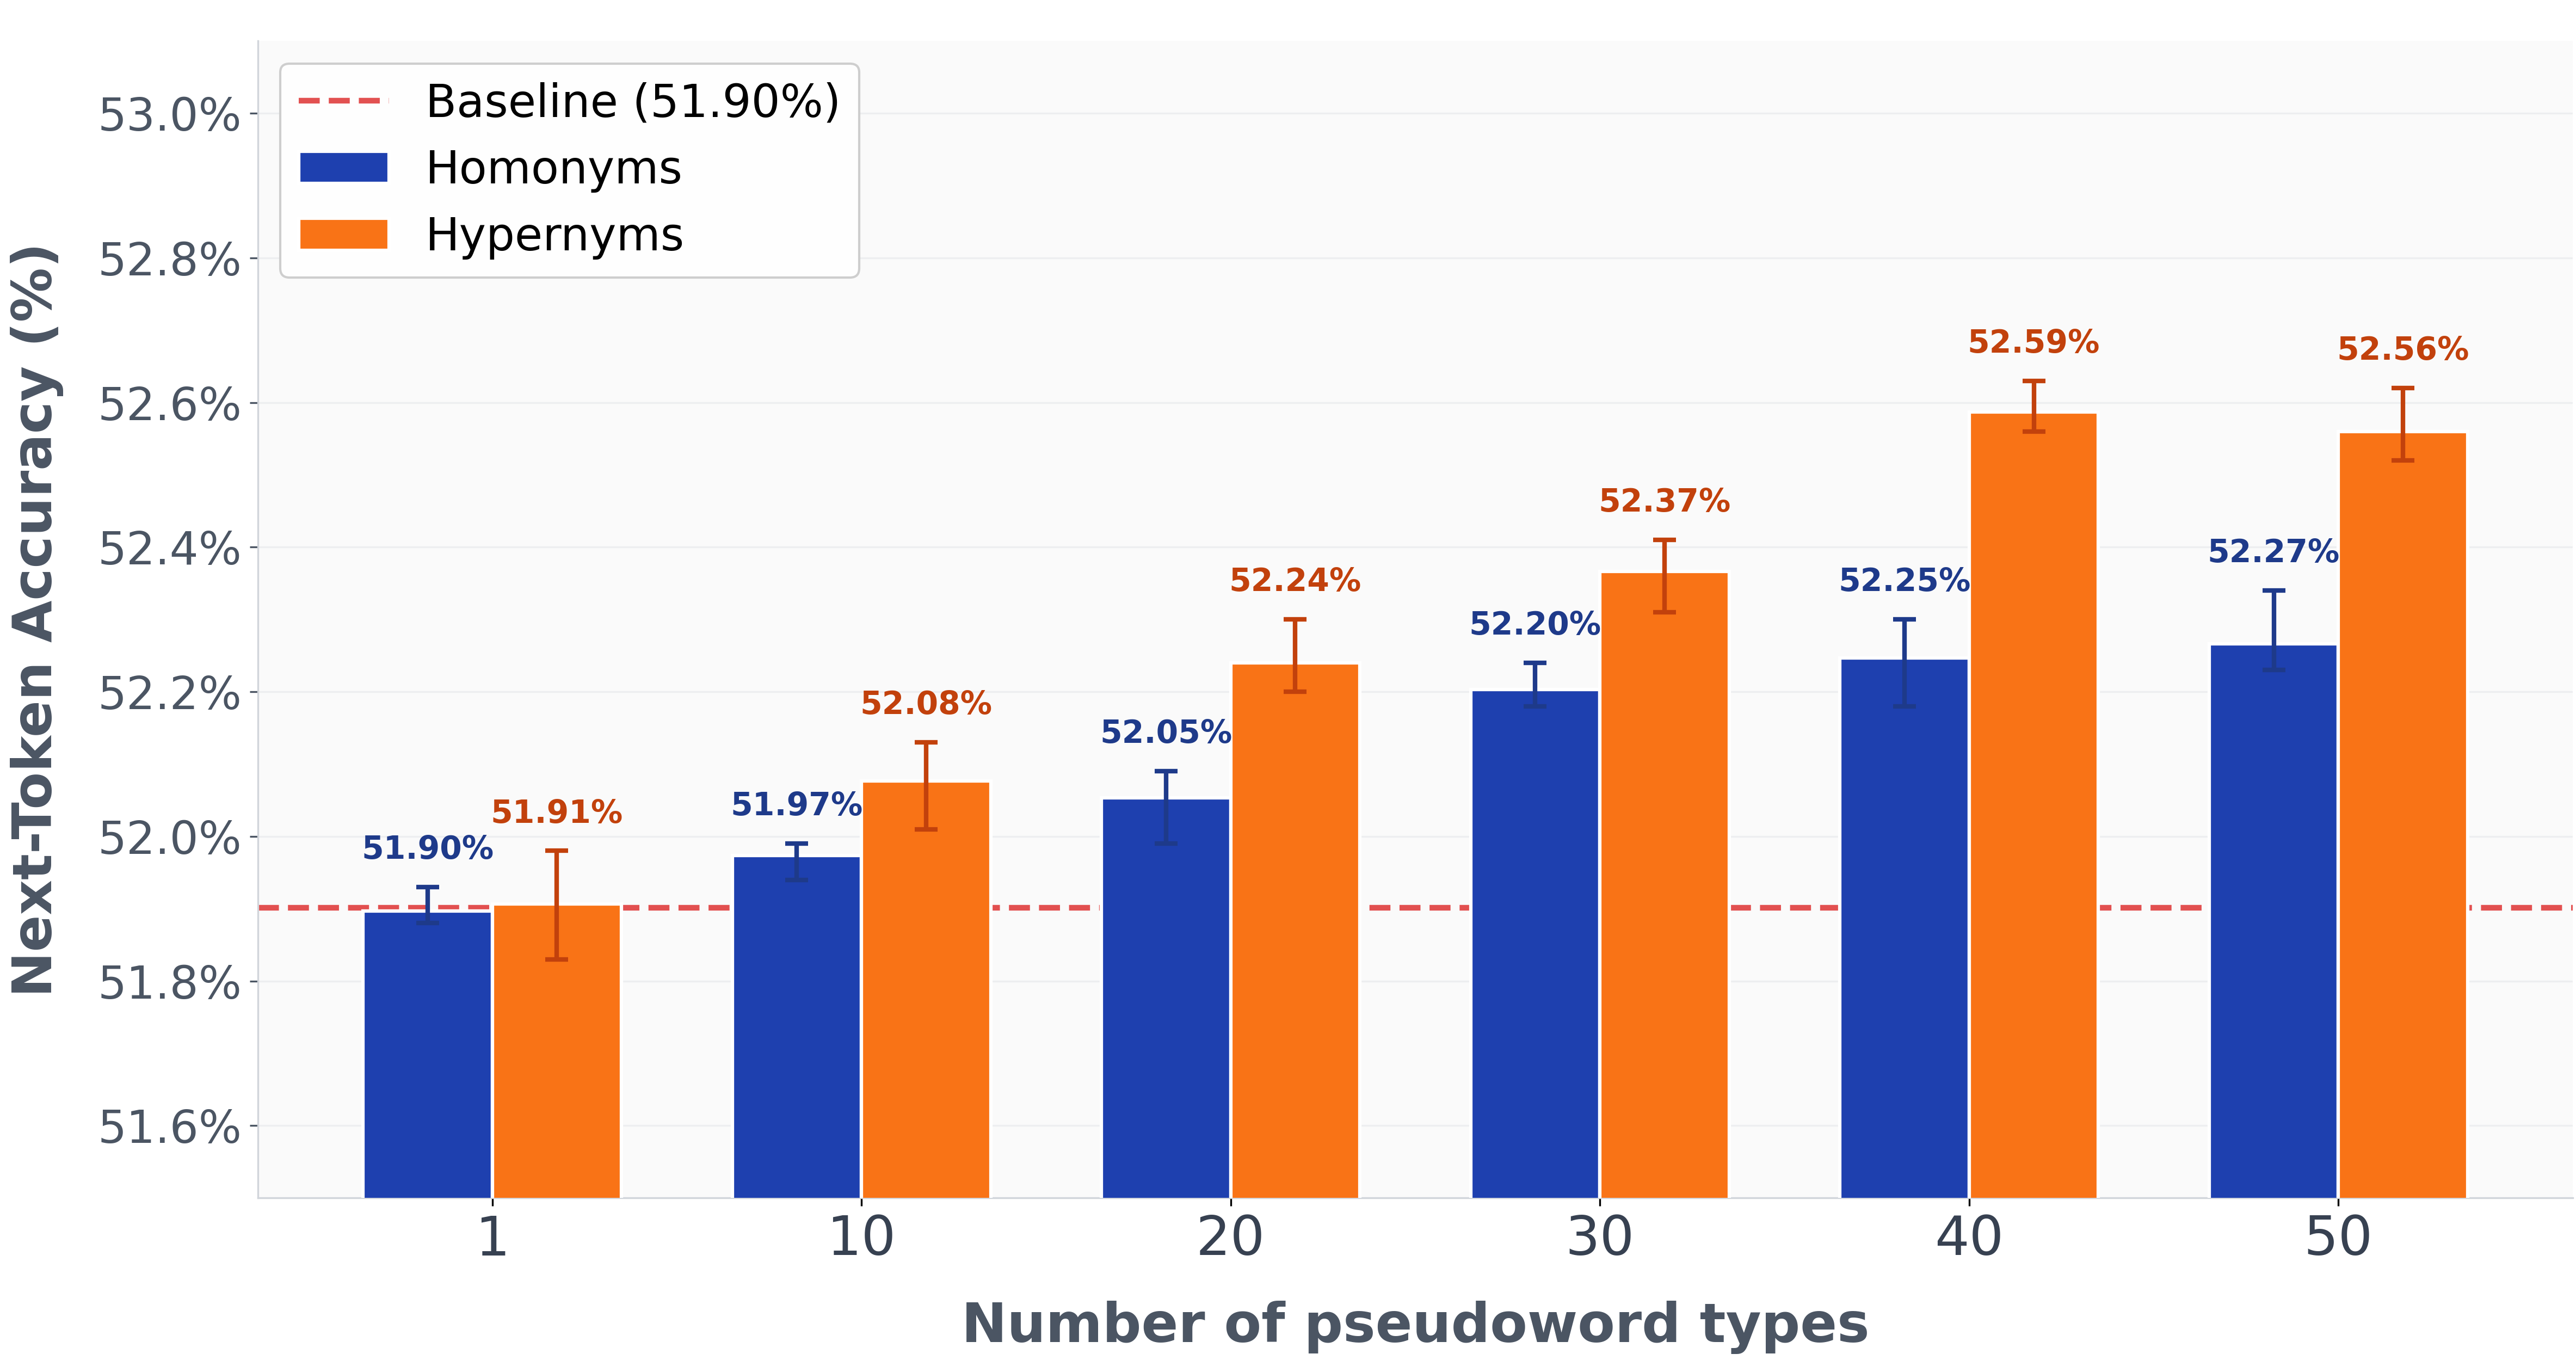
\includegraphics[scale=0.047]{images/recipe_homhyp.png}
 \caption{Accuracy for introducing pseudo-homonyms (HOM, left) and pseudo-hypernyms (HYP, right) into the RecipeNLG dataset, with 1--50 pseudoword types. Range bars show min/max over 3 runs; all HYP results and HOM results for n>10n>10
n>10 are significant (p<0.05p<0.05
p<0.05) compared to the baseline.}\label{fig:recipecomp}
\end{figure}
Results for the Recipe and Tiny Stories datasets are shown in Fig.~\ref{fig:recipecomp} and Fig.~\ref{fig:tinycomp}. In the domain-specific Recipe case, both types of pseudowords actually \emph{increase} model performance, with pseudo-hypernyms being particularly beneficial. The reason is intuitive: replacing two specific terms with one pseudoword reduces vocabulary variety, giving the model more capacity to learn each remaining word reliably, e.g., it no longer needs to distinguish \emph{mango} from \emph{papaya} and can learn just the pseudoword  \emph{papango}. Both pseudo-homonyms and pseudo-hypernyms achieve this effect, since their neighborhood distances are comparably high in the Recipe corpus (cf.\ Table~\ref{tab:neighborhood}), though pseudo-hypernyms offer a more practical form of compression because their components tend to be near-synonymous in context.
\begin{figure}
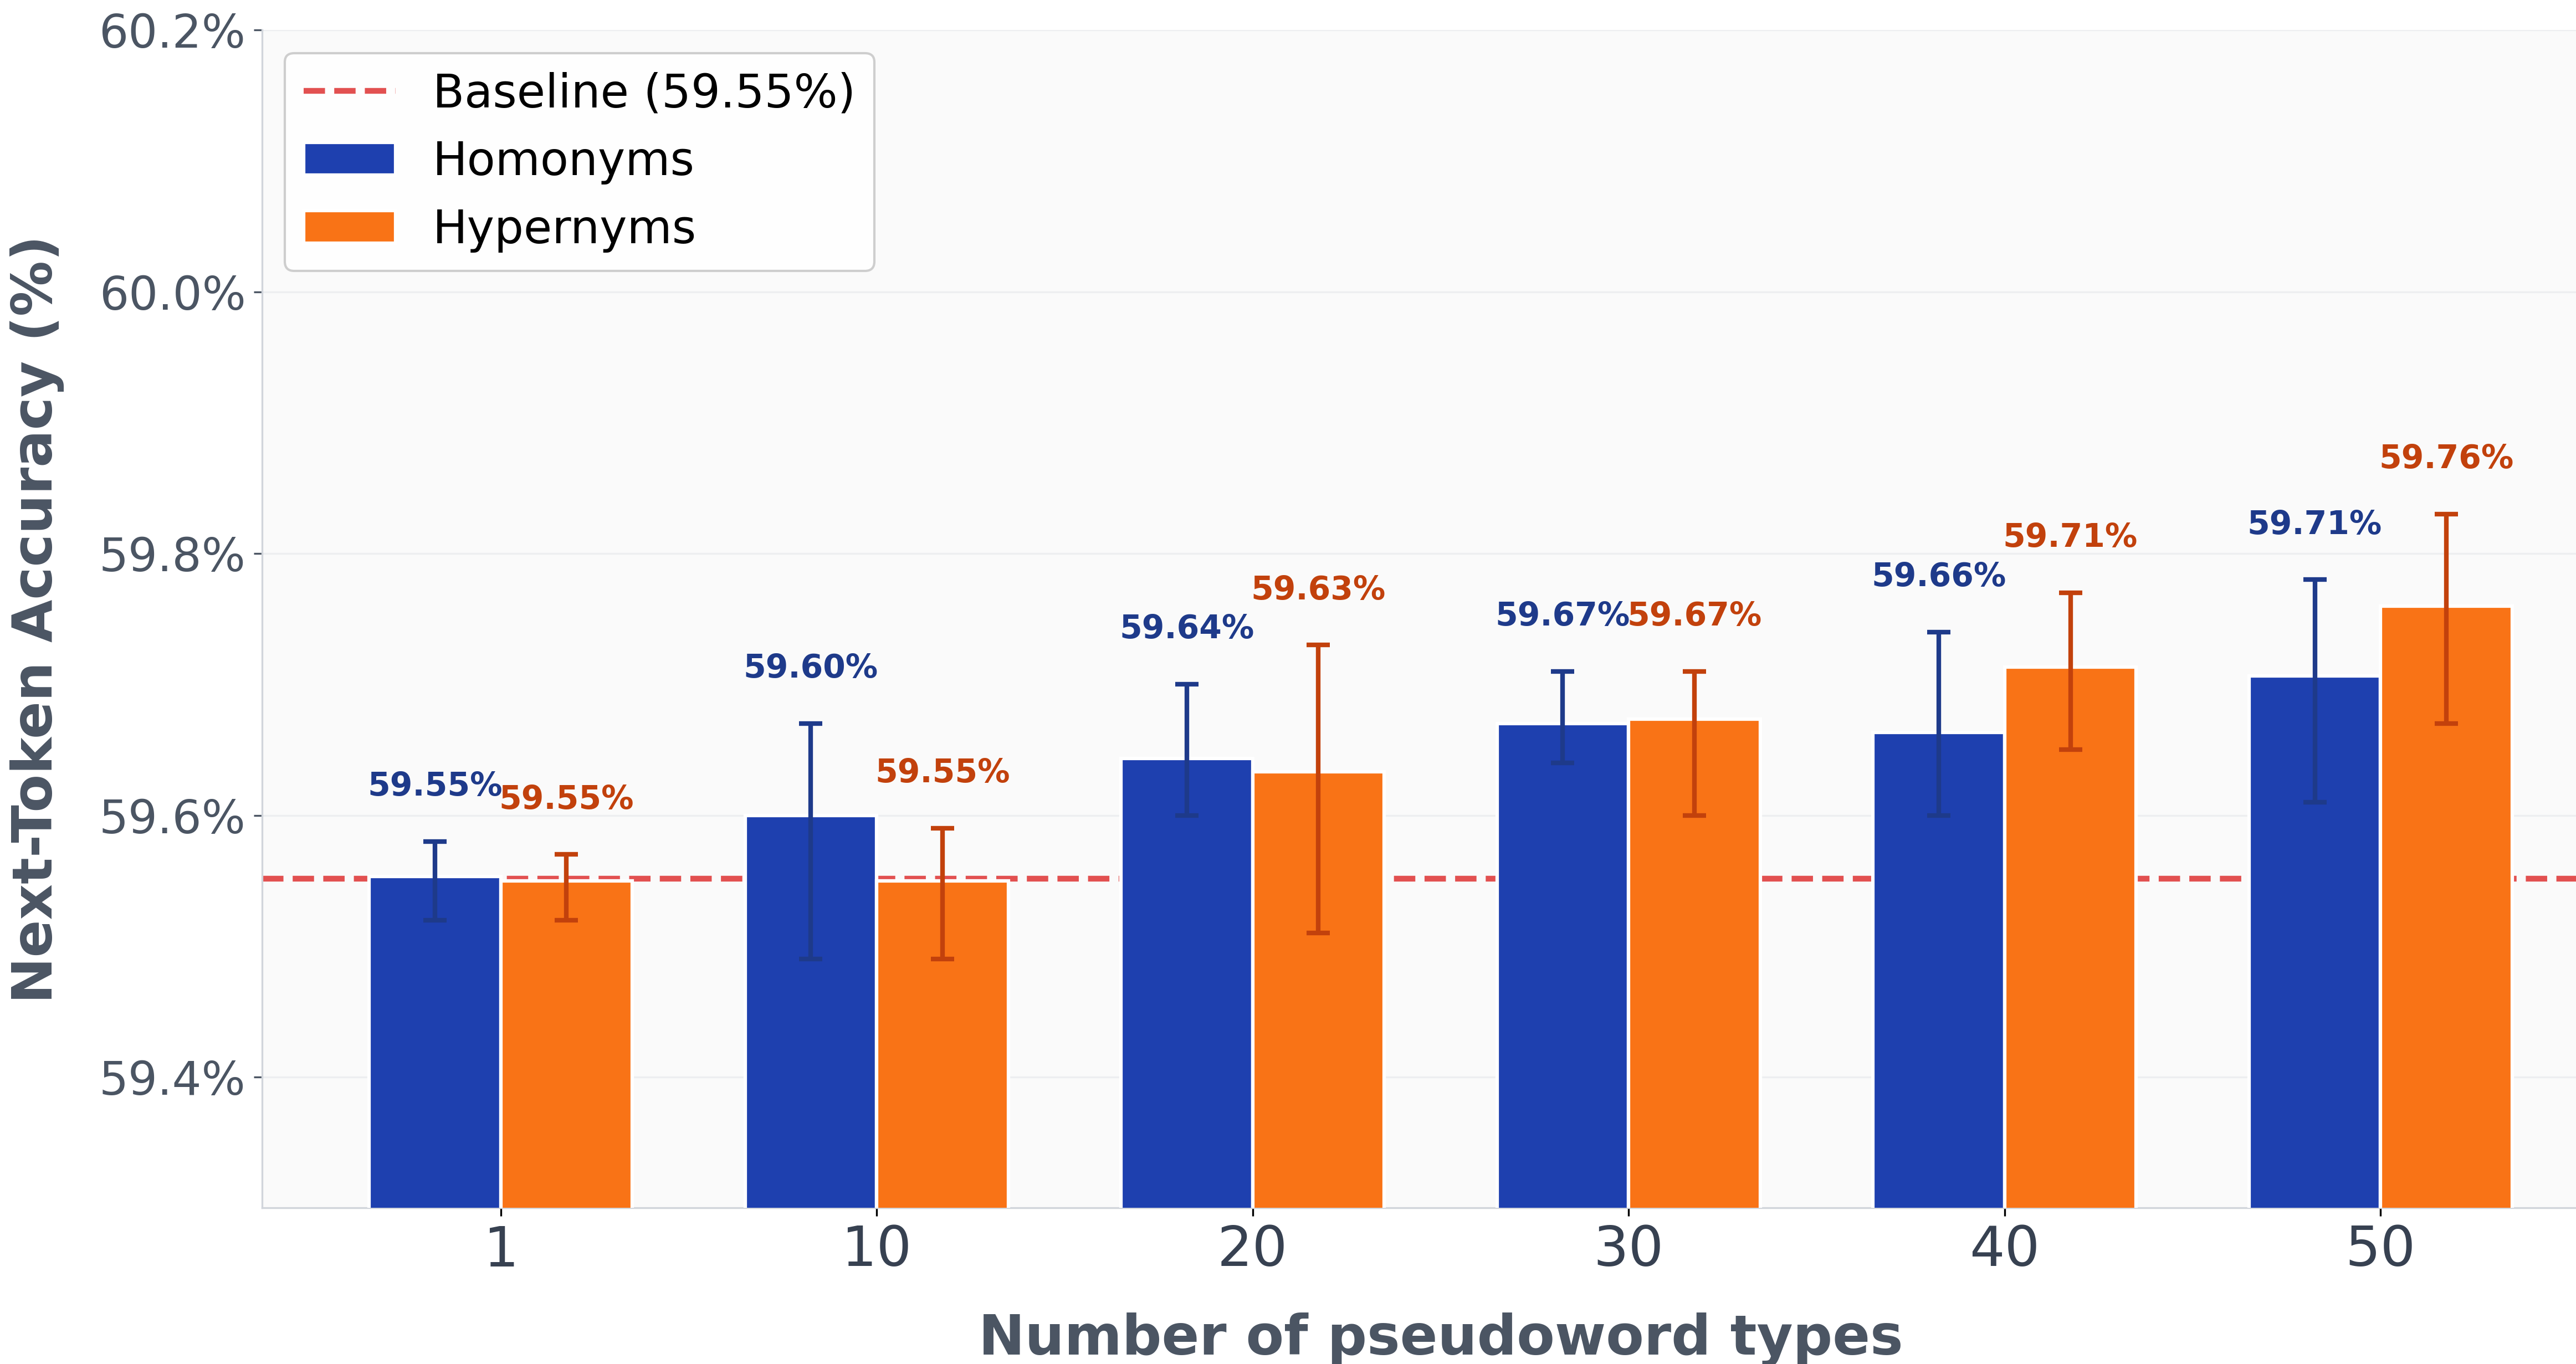
\includegraphics[scale=0.047]{images/tiny_homhyp.png}
\caption{Accuracy for introducing pseudo-homonyms (HOM) and pseudo-hypernyms (HYP) into the Tiny Stories dataset, with 1--50 pseudoword types. Range bars show min/max over 3 runs; no significant difference compared to the baseline.}\label{fig:tinycomp}
\end{figure}
On the Tiny Stories dataset, overall accuracy is higher, likely due to the smaller vocabulary and simpler syntax, but introducing pseudowords shows hardly any effect. The increase in performance is less pronounced, the variance across runs is higher, and we see no significant difference between pseudo-homonyms and pseudo-hypernyms despite their substantially different neighborhood distances — possibly because the high baseline variance masks smaller effects. Crucially, however, ambiguity does not \emph{decrease} performance: models handle increased lexical ambiguity at least as well as the unmodified baseline.
\emph{Takeaways: Introducing pseudo-homonyms and pseudo-hypernyms reduces vocabulary variety and increases model performance, especially for domain-specific texts. Ambiguity and underspecification can thus be effective means of compressing language models.}

\subsection{Adding Synonyms and Hyponyms}
In the previous experiment, we replaced all occurrences of the component words, creating a simpler scenario than natural ambiguity, where competing words remain in the text. In natural text, we would expect a homonym to coexist with synonyms indicating specific readings (e.g., \emph{club} as a synonym for one reading of \emph{bat}), and a hypernym to co-occur with its hyponyms. To model this more natural condition, we replace only half of the occurrences of each component word with the pseudoword, leaving the remaining sentences unchanged. (We randomly select half of the instances of each component, such that each component's frequency is halved uniformly.)
\begin{figure}
\centering
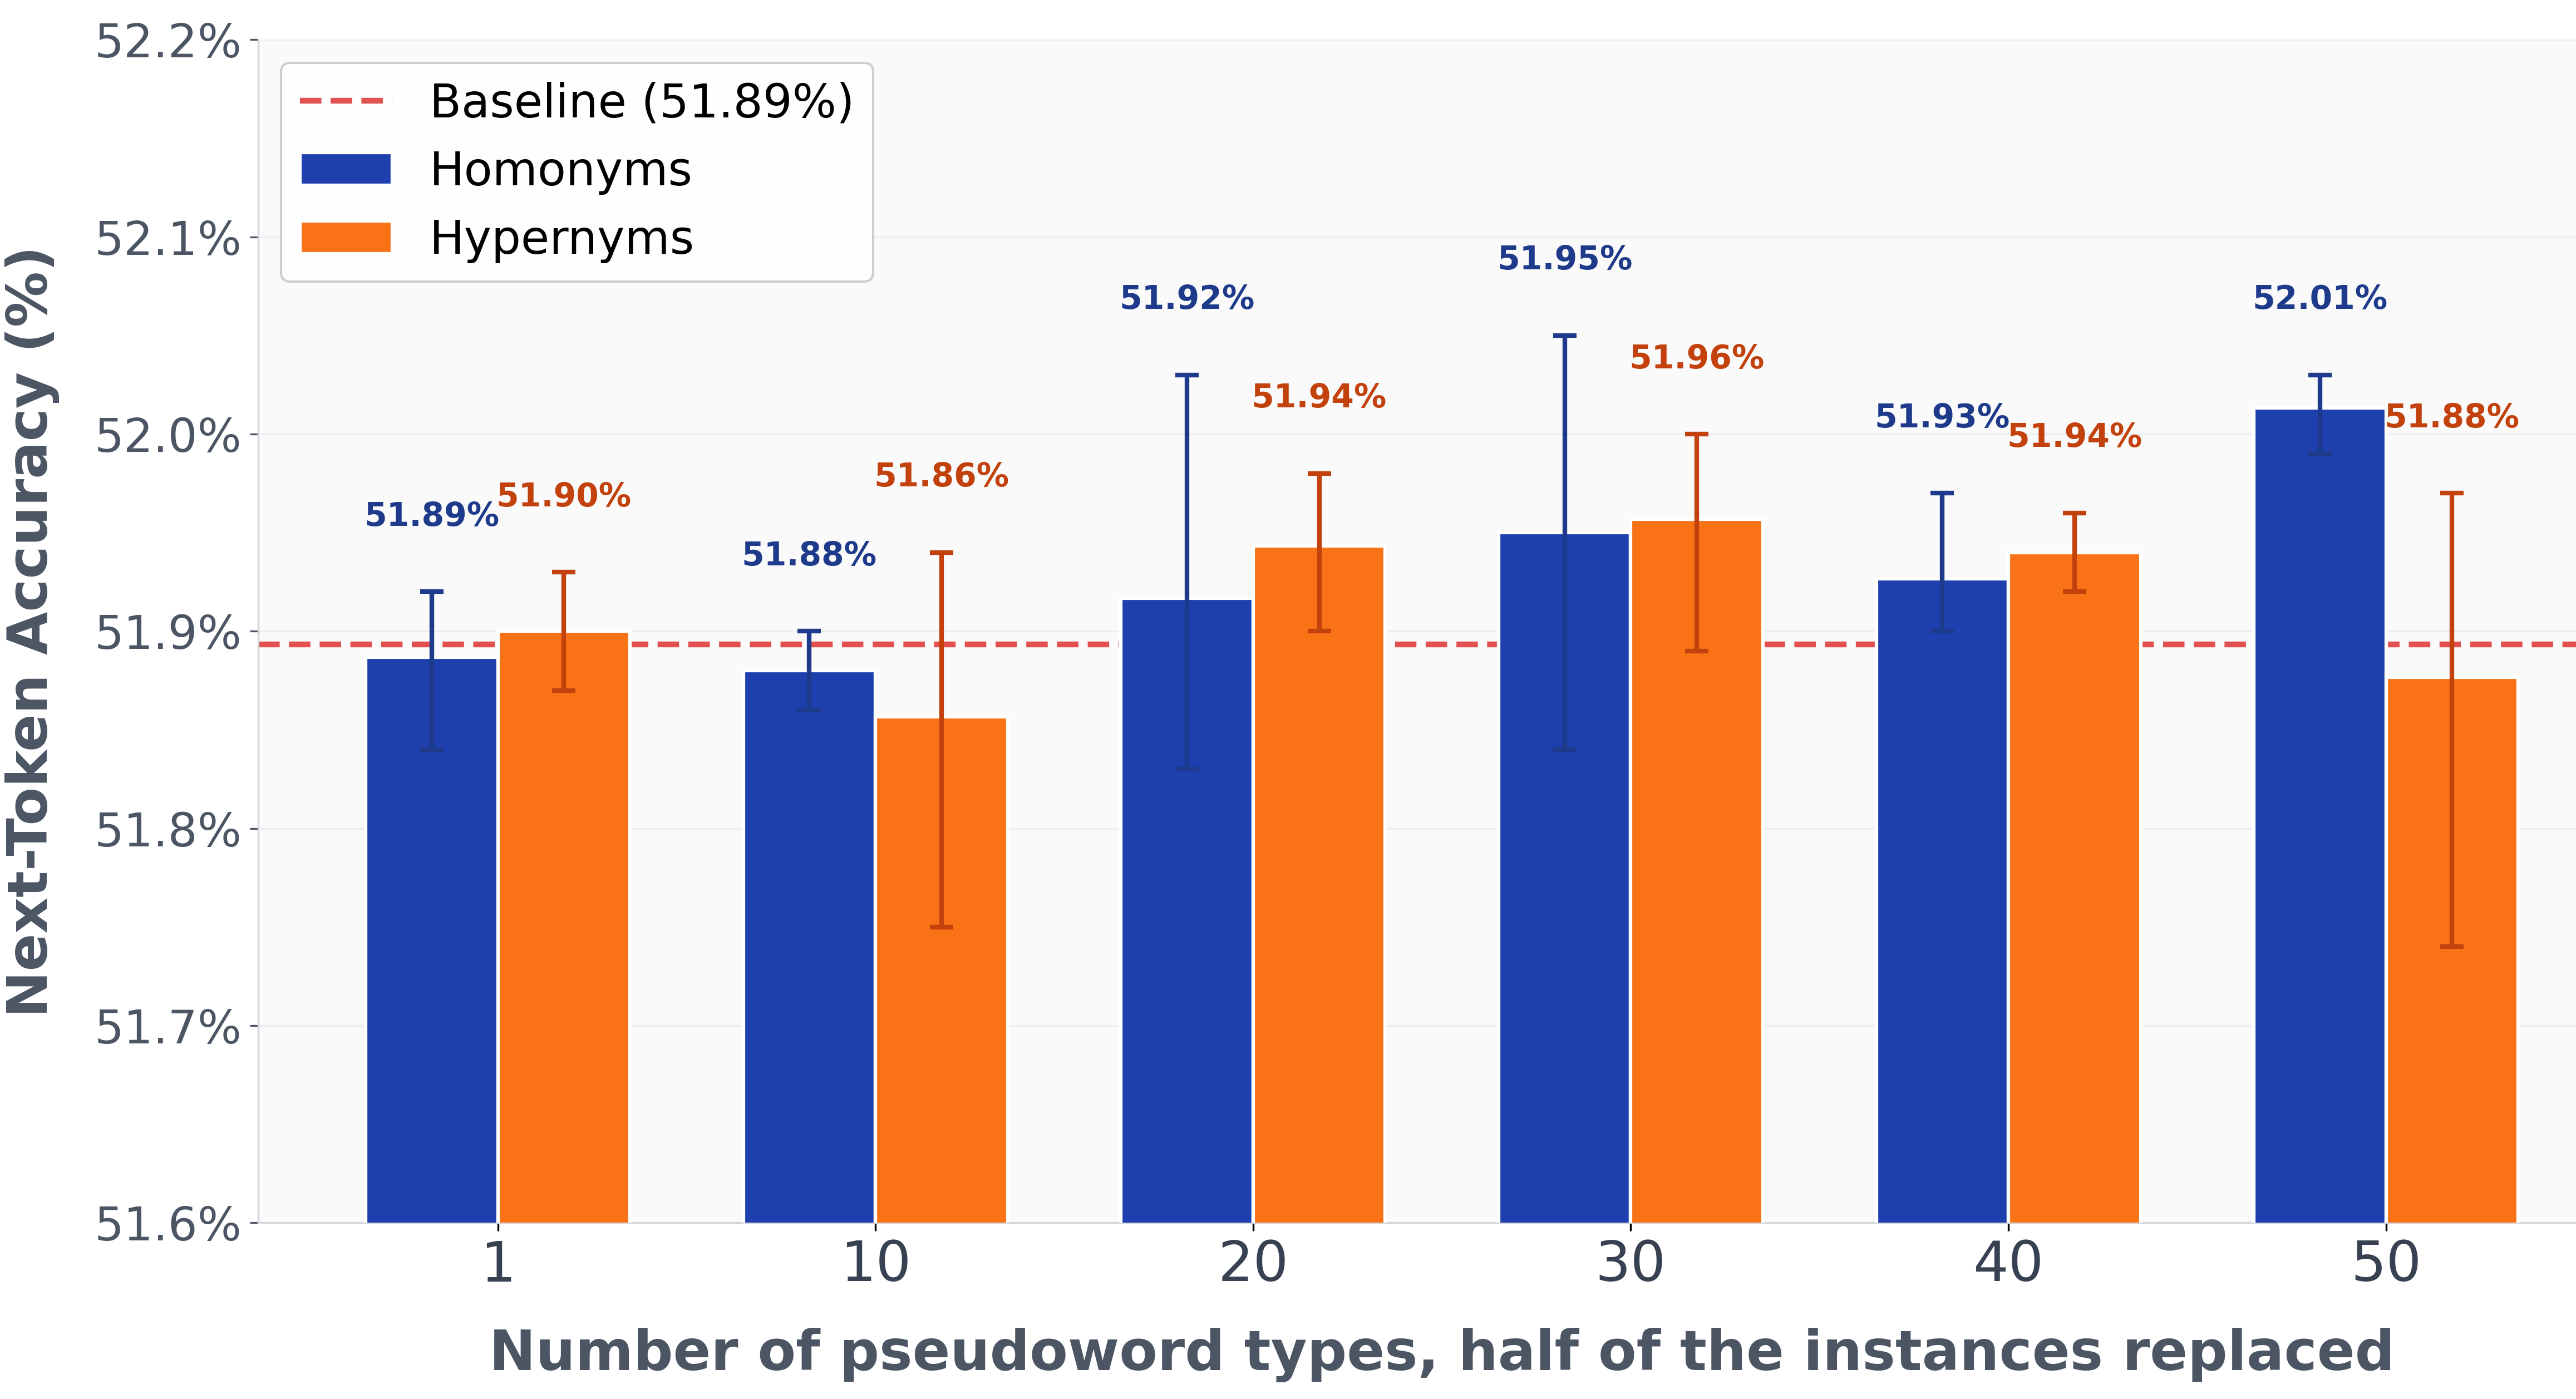
\includegraphics[scale=0.05]{images/recipe_half.png}
\caption{Accuracy for introducing pseudo-homonyms (HOM) and pseudo-hypernyms (HYP) into the RecipeNLG dataset, replacing only half of the pseudoword components, with 1--50 pseudoword types. Range bars show min/max over 3 runs; only HYP-50 shows a significant difference from the baseline.}\label{fig:recipehalf}
\end{figure}
Figures~\ref{fig:recipehalf} and~\ref{fig:tinyhalf} show the results for the Recipe and Tiny Stories datasets. The tendency of increasing accuracy with more pseudowords is no longer visible. This is expected, as two opposing effects are now intertwined: the vocabulary becomes more compact, but the model must additionally learn the relationship between each pseudoword and its surviving component words. For the Recipe dataset, we still observe a slight increase in accuracy with pseudo-hypernyms, but the effect is weaker than before and largely absent for pseudo-homonyms. On the Tiny Stories dataset, neither type shows a clear effect. We therefore examine the actual use of the pseudowords and their components in the next section.
\begin{figure}
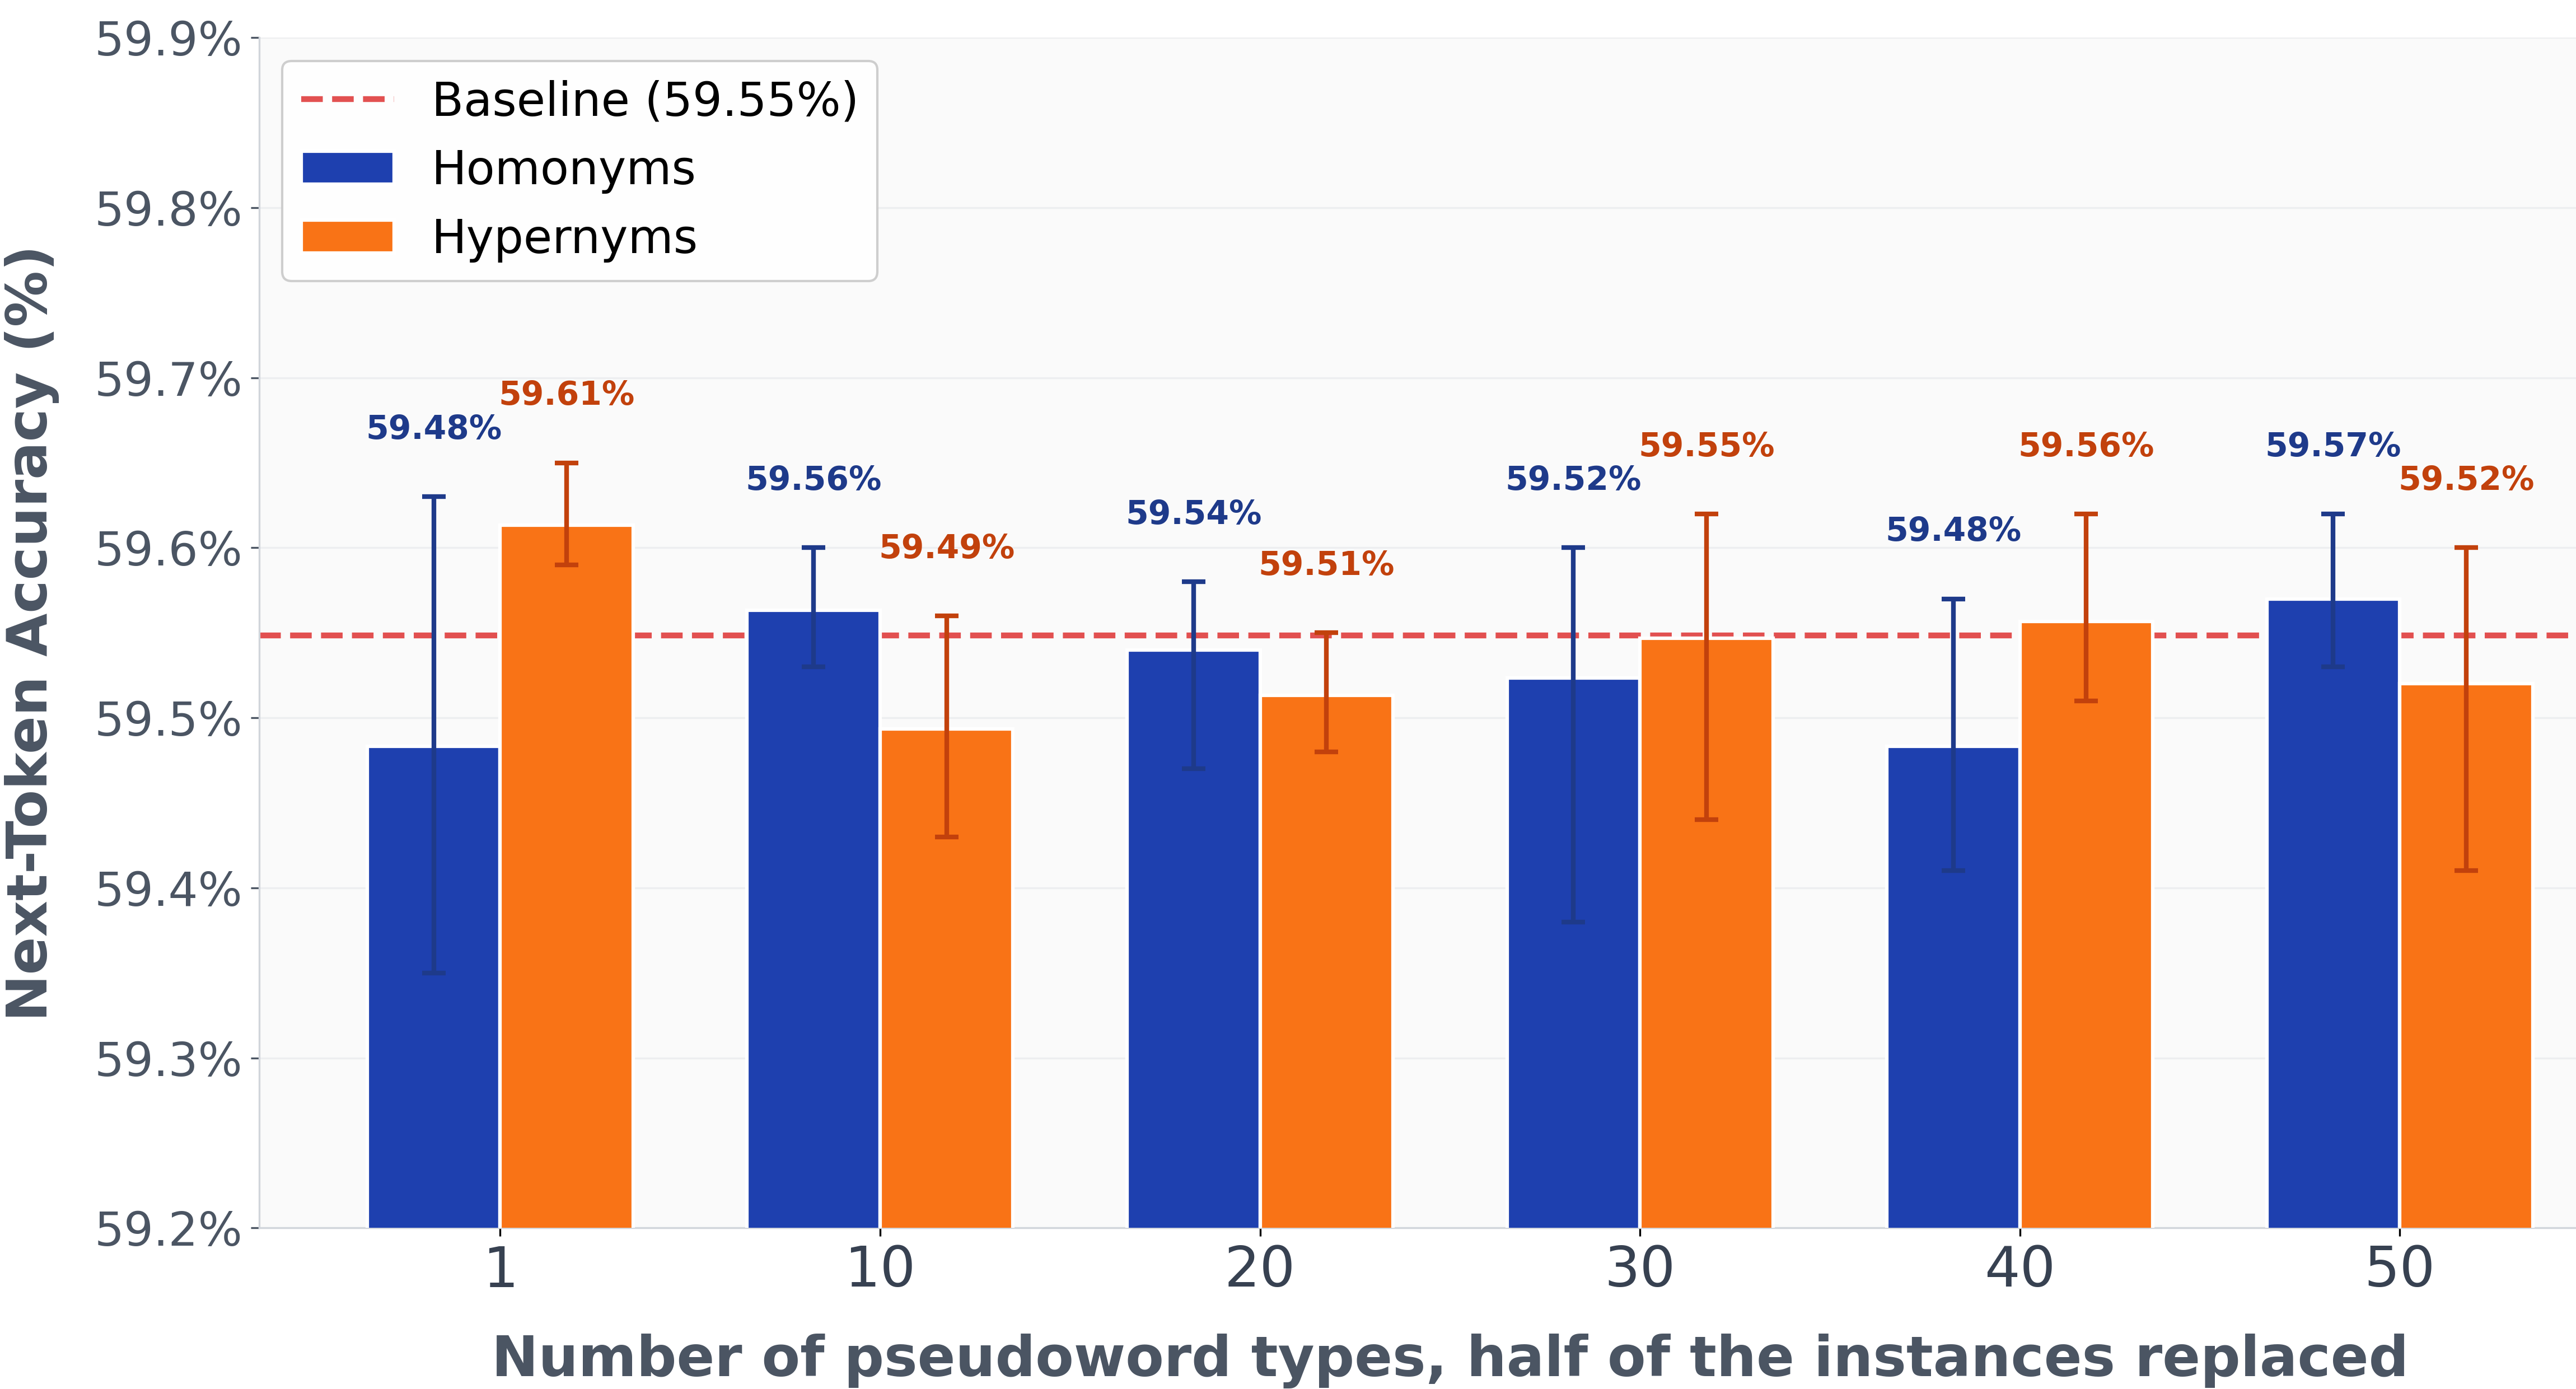
\includegraphics[scale=0.05]{images/tiny_half.png}
\caption{Accuracy for introducing pseudo-homonyms (HOM) and pseudo-hypernyms (HYP) into the Tiny Stories dataset, replacing only half of the pseudoword components, with 1--50 pseudoword types. Range bars show min/max across 3 runs; no significant difference from the baseline.}\label{fig:tinyhalf}
\end{figure}
\emph{Takeaways: The more natural setup with competing words (synonyms and hyponyms) diminishes the performance gains seen when all components are replaced. However, overall accuracy does not decrease below baseline, and pseudo-hypernyms can still yield modest gains in the domain-specific setting.}
\begin{figure*}
\centering
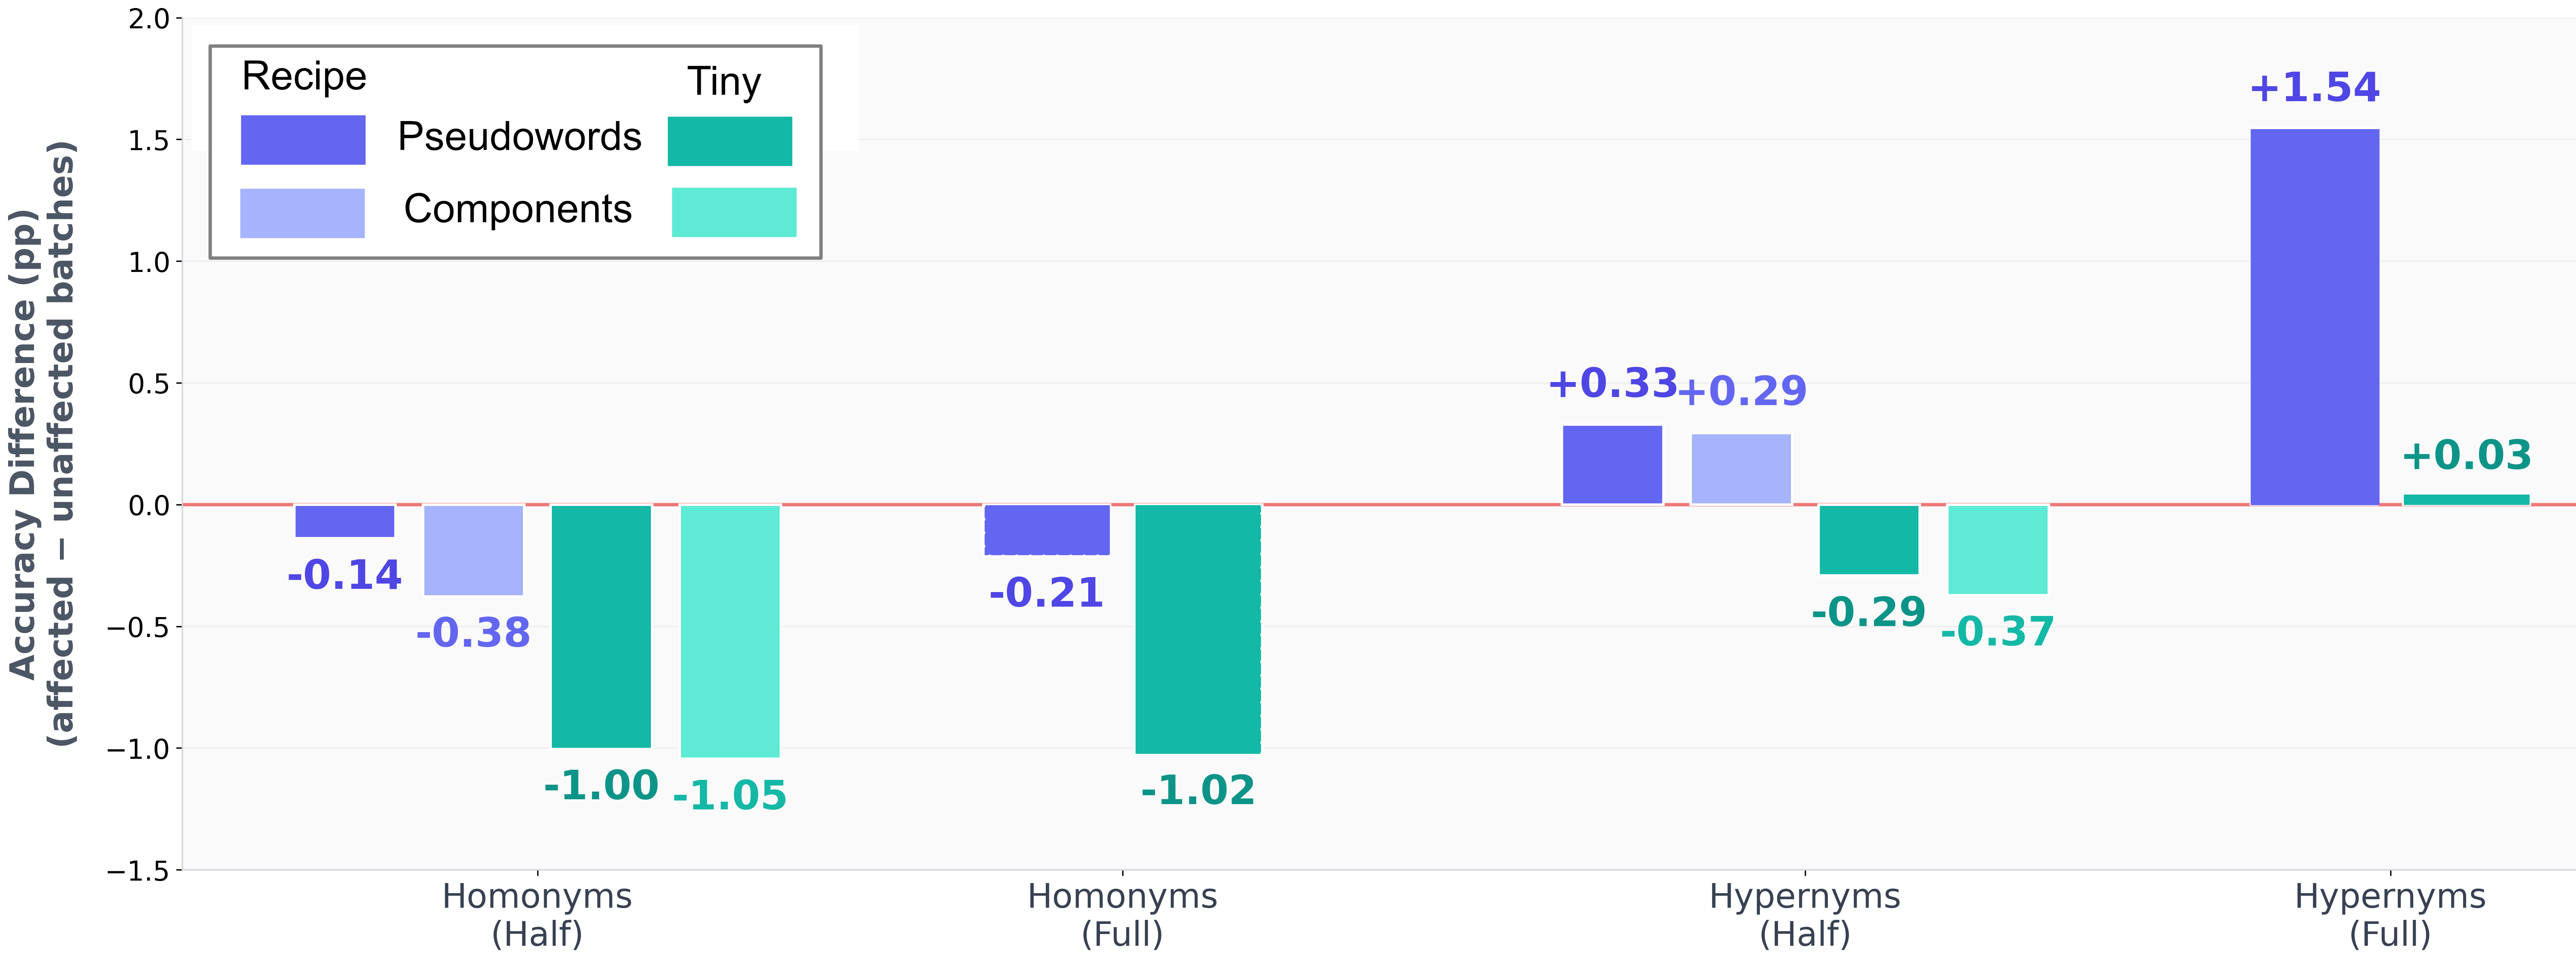
\includegraphics[scale=0.27]{images/component_eval.png}
\caption{Comparing accuracy for batches containing pseudowords or components with batches containing neither of them, using the models with 50 pseudoword types. The bars indicate the differences of the performance compared to batches without pseudowords or components. For the HALF models, we show both pseudowords and components next to each other; for the full models, only pseudowords. All results, except Recipe-Half/Pseudoword and Tiny-Full, are significant at $p<0.05$.}\label{fig:pseudocomp}

\end{figure*}
\subsection{Accuracy of Pseudowords and Their Components}
While the previous experiment showed that the presence of synonyms and hyponyms makes the language harder for the model to learn, overall performance did not decrease. To investigate in more detail, we conduct a finer-grained evaluation, separating validation batches into three groups: (1) batches containing at least one pseudoword, (2) batches containing at least one pseudoword component but no pseudoword (for the HALF models only), and (3) batches containing neither. This lets us assess whether the model can generate the pseudowords reliably, whether accuracy on surrounding tokens is affected, and whether the component words become harder to generate when competing with a pseudo-homonym or pseudo-hypernym. Note that we do not directly compare the accuracy of producing exactly the pseudowords or their components, since single-word accuracy is difficult to match against adequate controls. Instead, we use the accuracy on batches containing the target words as a proxy for the model's ability to generate them.
Figure~\ref{fig:pseudocomp} shows the results for both datasets. For the FULL models, we report the difference in accuracy between pseudoword batches and batches containing no pseudowords. For the HALF models, we additionally report results for batches containing at least one component word.
The results reveal a nuanced picture. Batches containing pseudo-homonyms or their components generally show lower accuracy than batches without them, though the effect is much more pronounced on the Tiny Stories dataset (right/green bars). For the domain-specific Recipe dataset, the drop is minimal and not significant for pseudoword batches. Pseudo-hypernyms, by contrast, tell a different story in the Recipe models: the models perform \emph{better} on both pseudoword batches and component batches. The pseudo-hypernyms are comparatively easy to learn and even seem to help the model learn the hyponyms when they are still present in the corpus (HALF condition). For Tiny Stories, pseudo-hypernyms are learnable when they fully replace their components, but accuracy on pseudoword batches decreases in the HALF condition. The effect is less pronounced than for pseudo-homonyms, but in both cases the component words suffer a greater accuracy loss than the pseudowords themselves. This mechanism could, at a larger scale, contribute to bias — for instance, introducing a general term like \emph{president} could make more specific terms like \emph{chairman} or \emph{chairwoman} harder to learn. We return to this point in Sec.~\ref{sec:discussion}.
\emph{Takeaways: Pseudo-homonyms are harder to learn than other vocabulary, and their components lose even more accuracy when both coexist in the corpus. Pseudo-hypernyms are easier to learn in domain-specific data but cause accuracy drops for components in general-language models, pointing to a potential source of bias at scale.}


\section{Discussion and Practical Implications} \label{sec:discussion}
Our results show how ambiguity and abstraction in training corpora affect the performance of the resulting models. We see several implications from our initial study for building responsible and performant LLMs:
\paragraph{Pseudo-hypernymy for model optimization:} While we aimed to show how much complexity ambiguity and abstraction add to model training, we find that pseudo-hypernyms actually increase model performance, especially for domain-specific texts. 
This suggests a concrete optimization strategy for more sustainable LLM design: if the distinction between specific terms is irrelevant for the target task (e.g., in classification scenarios), replacing co-hyponyms with pseudo-hypernyms can compress both the training data and the model, yielding better performance with fewer resources. This approach seems particularly promising for domain-specific texts, where we observe the largest gains. While large-scale feasibility requires further research, this could be a promising direction for LLMs optimization in downstream tasks.
\paragraph{Learning of ambiguous words and their synonyms:} Our experiments show that ambiguity alone does not harm model performance; rather, the harm arises when ambiguous words coexist with synonyms that correspond to only one of their readings. To some degree, we see the same effect for pseudo-hypernyms in open-domain language. This means that efforts to improve model outputs with respect to both ambiguity handling and fairness cannot be restricted to the ambiguous or underspecified terms themselves but must take all related words into account. Future research needs to show whether such performance deficits lead to bias propagation, e.g., that the default resolution of \emph{director} to a male person also biases the generation of related terms like \emph{bank manager} towards male-associated contexts.
%\paragraph{Influence of domain specificity:} Domain specificity has a large influence on ambiguity handling. While a specific domain still features homonyms, their new introduction is less harmful than in a general-domain corpus, even when that corpus has restricted vocabulary and is overall easier for the model to process. This also means that general model performance on a corpus is not indicative of the model's capability for handling ambiguity and abstraction.
\section{Conclusion} \label{sec:conclusion}
We evaluated the effects of ambiguity and abstraction on language model performance by using pseudowords as pseudohomonyms or pseudohypernyms. We showed that increasing the number of pseudohomonyms or pseudohypernyms does not harm model performance per se, and that replacing specific words with pseudohypernyms can increase performance due to the reduction in vocabulary variety. When examining the models' ability to generate ambiguous or underspecified words, however, we find that in settings where synonyms or individual hyponyms still occur in the training corpus, both the pseudowords and their component words are generated less reliably than other vocabulary.
While our study focuses on small models and small language modifications, we observe statistically significant effects that point to concrete implications for responsible LLM design. On the one hand, models can be compressed by reducing vocabulary variety through the principle of abstraction. Replacing words that are related in vector space with a single pseudoword improves model performance, yielding more sustainable and compact models, especially for downstream tasks such as classification that do not depend on open-ended generation. On the other hand, ambiguity and abstraction can harm performance for both the underspecified expressions and their hyponyms or individual readings. This means that research on fairness and bias must take into account not only expressions like \emph{manager} but also their hyponyms and related terms.
In future work, we aim to show how the effects we observe scale to larger models and larger vocabulary modifications, and how performance drops from increasing ambiguity can be mitigated — for instance through targeted data balancing or training strategies that account for the semantic relationships between pseudowords and their components.
\section*{Limitations}
Our experiments comprise many individual language models based on several modifications of two base corpora. While this provides an in-depth analysis, the scope is limited in several respects:
\paragraph{Model choice:} All our models are GPT-2 models trained from scratch. While we believe that our results carry over to other model families, this remains to be verified. Further, to avoid confounders, we did not optimize hyperparameters individually for each run; some effects might change with hyperparameter tuning.
\paragraph{Ambiguity and abstraction:} With pseudohomonyms and pseudohypernyms, we study only one type of ambiguity and one type of abstraction. Both phenomena occur at multiple linguistic levels that interact with each other, and we have only examined a small subset that we could cover with pseudowords. Future work will need to present experimental setups that accommodate different types of ambiguity, such as syntactic or discourse-level ambiguity.
\paragraph{Scaling and evaluation:} To isolate effects of small language changes, we used small language models and restricted corpora. Future work needs to scale our findings to larger models, different domain-specific corpora, and more general corpora. In those settings, established benchmarks (e.g., HellaSwag) can be used to test the impact of ambiguity; such benchmarks are not meaningful for our small models, so we rely on next-token prediction accuracy as our sole evaluation metric. Scaling up will also show whether our assumption holds that models compressed through pseudohypernyms still perform well on downstream tasks.
\section*{Ethical Considerations}
Our research can contribute to more sustainable model development: we provide initial evidence that linguistically motivated compression of LLMs is feasible, showing that pseudohypernyms can reduce vocabulary variety and improve performance, especially for domain-specific models. If these findings scale, they could reduce the computational resources and energy required for model training. We also believe our results can inform research on fairness, since we show that the introduction of ambiguous or underspecified terms can degrade accuracy not only for those terms but also for their related words — a mechanism that, at scale, could contribute to bias propagation in ways that are difficult to detect by examining individual terms in isolation.
\bibliographystyle{compling}
\bibliography{ambiguity}




\end{document}

